\section{Resultados e Discussão}
Este capítulo apresenta discussões acerca dos resultados obtidos nos experimentos dos algoritmos. O conteúdo divide-se em duas seções. A primeira sessão aborda os resultados das simulações envolvendo o processo de construção dos rastros de feromônio e detecção e propagação dos eventos. A segunda demonstra os resultados das simulações ao se adicionar o comportamento de reforço da conectividade da rede, onde são apresentados os resultados da combinação das estratégias, bem como os resultados da utilização independe do último algoritmo.

\subsection{Construção dos Rastros de Feromônio e Propagação de Eventos}
Os experimentos realizados para avaliar o desempenho da técnica desenvolvida no trabalho foram baseados na comparação desta técnica com uma abordagem tradicional: o envio de mensagens por \emph{flooding}. No caso da propagação de mensagens por \emph{flooding}, quando um evento é detectado, o nó sensor detector envia o alarme em \emph{broadcast} e todos os seus vizinhos repetem este alarme (também em \emph{broadcast}), de modo que todos os nós do sistema repitam o alarme, até que, em algum momento, a mensagem chegue ao \vant de destino.

As métricas avaliadas nesta comparação foram:

\begin{description}
\item[a) Número total de Mensagens: ] representa o número total de mensagens utilizadas para enviar um alarme até seu destinatário.
\item[b) Número de Saltos:] o número de saltos realizados por um alarme desde seu emissor até seu receptor. Este valor representa a quantidade de nós intermediários entre o nó emissor e o \vant receptor do alarme.
\end{description}

\subsection{Configurações da Simulação}
Foram realizadas 200 simulações (100 simulações em cada técnica). Os experimentos foram realizados com o intuito de avaliar o comportamento da rede de forma isolada no acontecimento de um evento de interesse. Portanto, optou-se por simular um cenário contendo apenas um \vant e com a ocorrência de apenas um evento de interesse, de modo que se consiga visualizar o comportamento específico do envio de mensagens através do \emph{backbone} sem a interferência de muitos eventos. O intervalo de tempo em que as métricas são analisadas é o tempo necessário para a ocorrência de um evento em adição ao tempo gasto para que a mensagem alcance seu destino.

A escolha dos parâmetros de configuração da simulação, em relação às capacidades dos \vants, foi determinado baseando-se no uso de Mini e Micro-\vants. Baseando-se nas informações em \cite{uas_2009,Storvold2009}, optou-se por uma altitude de 250 metros. Em relação aos nós sensores terrestres, foram simuladas as funcionalidades de rádios do tipo IEE 802.15.4.

Neste cenário, quando um \vant não está respondendo a um alarme, deve realizar sua rota de forma aleatória, de modo a construir seu rastro de feromônio. São distribuídos 140 nós sensores terrestres (com raio de comunicação de 300m) seguindo a distribuição de Poisson em uma área de 2Km x 2km, obtendo-se aproximadamente 100\% de probabilidade de que os nós formem um grafo conexo \cite{Bettstetter2002}.

A tabela \ref{tbl:setup} resume os parâmetros das simulações.

\begin{table}[h!]
\centering
	\begin{tabular}{| l | l |}
		\hline
		Parâmetro & Valor \\
		\hline
		Cenário & 2 Km x 2 Km\\
		Raio de Comunicação do \vant & 400m\\
		Altitude de Vôo & 250m  \\
		Número de nós sensores estáticos & 140  \\
		Raio de comunicação dos nós sensores & 300m \\
		\hline
	\end{tabular}

	\caption{Parâmetros para simulação da Construção dos Rastros de Feromônio e Propagação de Eventos.}
	\label{tbl:setup}
\end{table}


\subsubsection{Resultados}

 A figura \ref{fig:hops} demonstra os resultados da simulação em relação ao número de saltos ocorridos até que o \vant recebesse o alarme. O eixo x representa o número da simulação e o eixo y representa o número de saltos necessário para que o alarme alcançasse o destino. Pode-se notar uma proximidade nestes resultados em relação aos valores, isto deve-se ao fato de que esta métrica avalia o caminho percorrido pelo alarme em um mesmo cenário para ambas as simulações. É importante verificar que no algoritmo baseado em feromônios, a mensagem percorre um único caminho até alcançar seu receptor. Em contrapartida, na estratégia baseada em \emph{flooding}, são percorridos todos os possíveis caminhos contidos no grafo formado pelos nós sensores. Isto implica que em um determinado momento, dentre todos os caminhos, um deles encontrará o \vant. Neste caso, o número de saltos com valores próximos é justificado pelo fato de que um dos caminhos encontrados na estratégia de \emph{flooding} (exatamente o caminho que foi contabilizado no experimento) é um caminho muito parecido com o utilizado pelo algoritmo de feromônio. A figura \ref{fig:hops_mean} apresenta a média dos resultados para este experimento.


 \begin{figure}[h!]
 \centering
 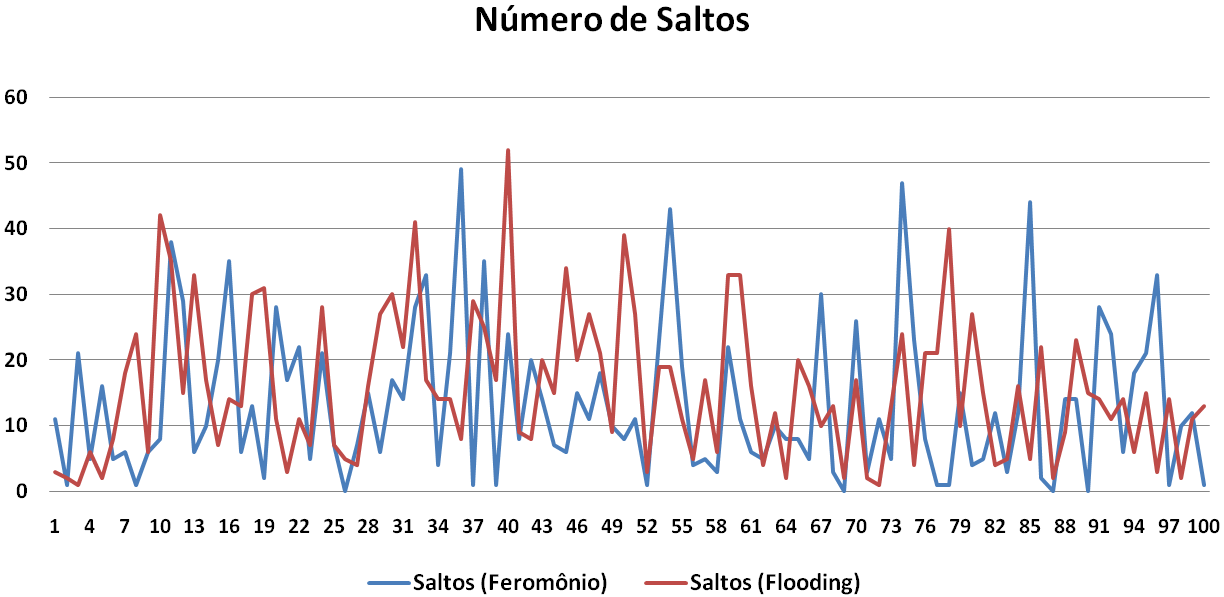
\includegraphics[width=13cm]{results/hops.png}
 \caption{Resultados em relação ao número de saltos.}
  \label{fig:hops}
 \end{figure}


 \begin{figure}[h!]
 \centering
 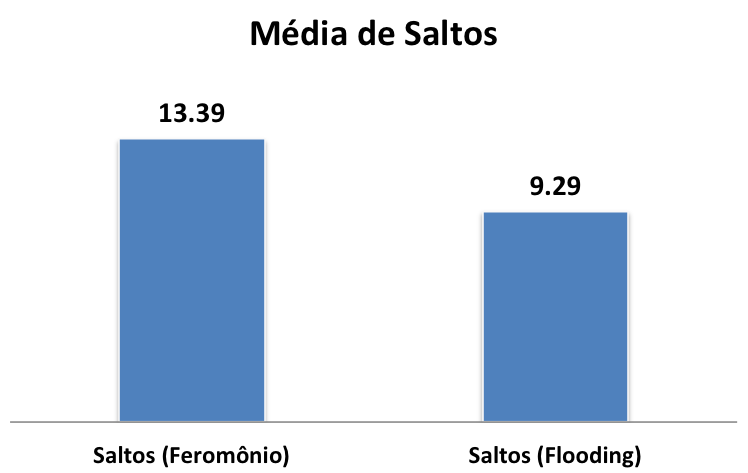
\includegraphics{results/hops_mean.png}
 \caption{Média do Número de Salto.}
  \label{fig:hops_mean}
 \end{figure}

Os resultados anteriores não justificam a utilização do algoritmo de feromônios. Contudo, ao se analisar os resultados em relação ao número de mensagens enviadas, é possível verificar a eficiência deste algoritmo em relação ao método tradicional de \emph{flooding}. As figuras \ref{fig:messages} e \ref{fig:messages_mean}, respectivamente, exibem os resultados obtidos em cada simulação e a média do número de mensagens enviadas pelo sistema durante a entrega de um alarme. Nota-se uma relação na ordem de aproximadamente 9,7 vezes nos resultados para o número de mensagens. Este resultado complementa os dados apresentados anteriormente, mostrando a real diferença entre as duas técnicas. A diferença pode ser vista pelo fato de que, mesmo realizando valores de saltos muito próximos, os algoritmos diferenciam-se na quantidade utilizada de mensagens para a entrega de um alarme. O uso do rastro de feromônio garante que somente um caminho será tomado para a busca do \vant, ao contrário da abordagem tradicional, onde todos os possíveis caminhos são verificados.

 \begin{figure}[h!]
 \centering
 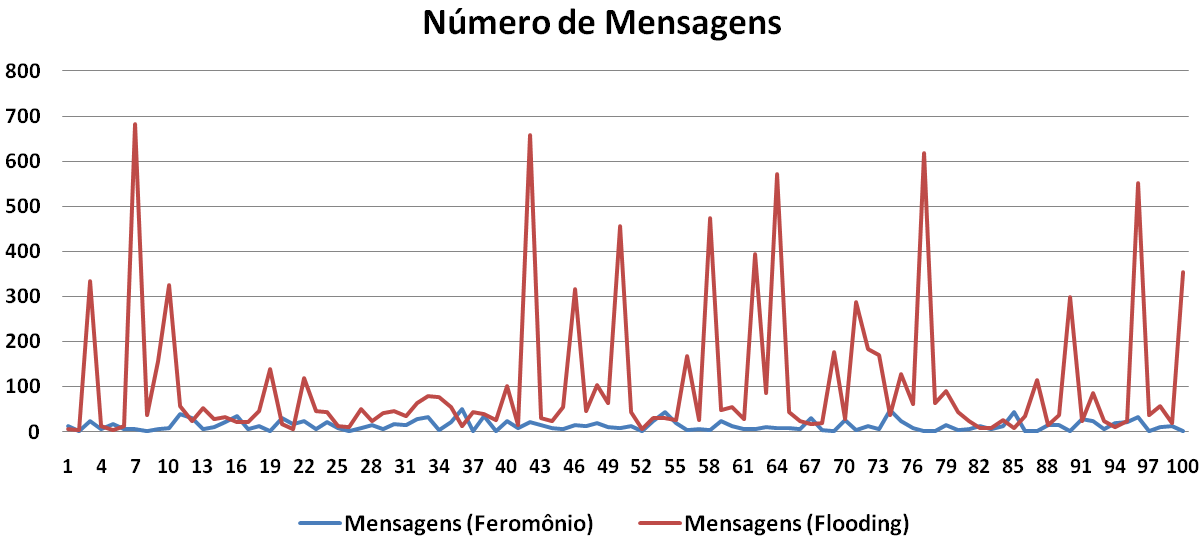
\includegraphics[width=13cm]{results/messages.png}
 \caption{Resultados em relação ao número de mensagens enviadas.}
  \label{fig:messages}
 \end{figure}

 \begin{figure}[h!]
 \centering
 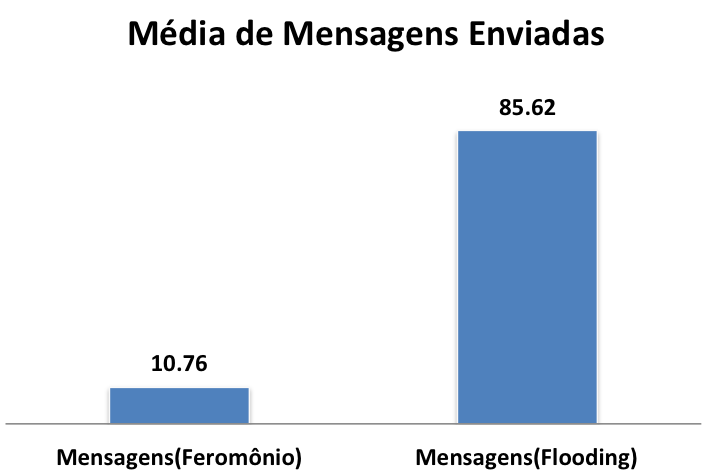
\includegraphics{results/messages_mean.png}
 \caption{Média do Número de Mensagens.}
  \label{fig:messages_mean}
 \end{figure}

Os resultados demonstram a possibilidade de se reduzir o número de mensagens trafegadas em uma rede de sensores sem fio no que se refere a detecção e propagação de eventos em uma área de interesse. Observando-se o gráfico \ref{fig:global_mean}, tem-se o resultado geral da simulação, onde podem ser visualizados os resultados anteriores em uma mesma escala.

\begin{figure}[h!]
 \centering
 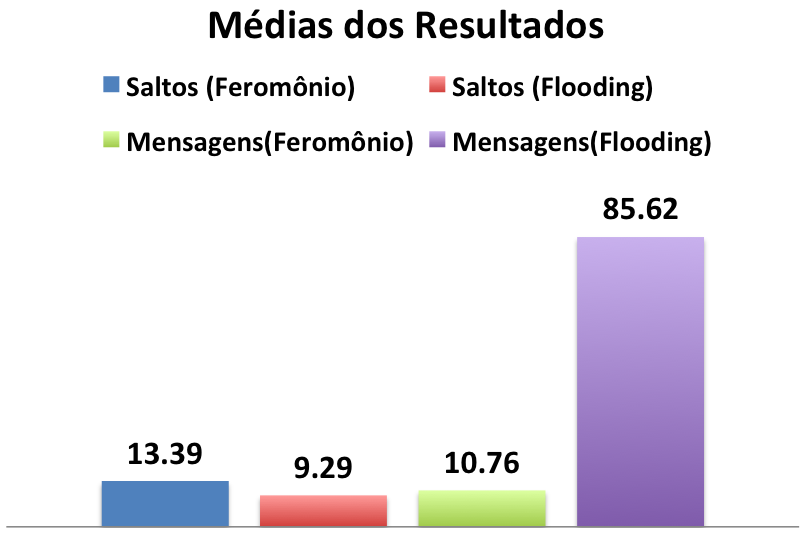
\includegraphics{results/global_mean.png}
 \caption{Média geral dos resultados.}
  \label{fig:global_mean}
 \end{figure}

A próxima seção discute os resultados do segundo algoritmo proposto por este trabalho. 
